\documentclass[]{elsarticle} %review=doublespace preprint=single 5p=2 column
%%% Begin My package additions %%%%%%%%%%%%%%%%%%%
\usepackage[hyphens]{url}
\usepackage{lineno} % add
\providecommand{\tightlist}{%
  \setlength{\itemsep}{0pt}\setlength{\parskip}{0pt}}

\bibliographystyle{elsarticle-harv}
\biboptions{sort&compress} % For natbib
\usepackage{graphicx}
\usepackage{booktabs} % book-quality tables
%% Redefines the elsarticle footer
%\makeatletter
%\def\ps@pprintTitle{%
% \let\@oddhead\@empty
% \let\@evenhead\@empty
% \def\@oddfoot{\it \hfill\today}%
% \let\@evenfoot\@oddfoot}
%\makeatother

% A modified page layout
\textwidth 6.75in
\oddsidemargin -0.15in
\evensidemargin -0.15in
\textheight 9in
\topmargin -0.5in
%%%%%%%%%%%%%%%% end my additions to header

\usepackage[T1]{fontenc}
\usepackage{lmodern}
\usepackage{amssymb,amsmath}
\usepackage{ifxetex,ifluatex}
\usepackage{fixltx2e} % provides \textsubscript
% use upquote if available, for straight quotes in verbatim environments
\IfFileExists{upquote.sty}{\usepackage{upquote}}{}
\ifnum 0\ifxetex 1\fi\ifluatex 1\fi=0 % if pdftex
  \usepackage[utf8]{inputenc}
\else % if luatex or xelatex
  \usepackage{fontspec}
  \ifxetex
    \usepackage{xltxtra,xunicode}
  \fi
  \defaultfontfeatures{Mapping=tex-text,Scale=MatchLowercase}
  \newcommand{\euro}{€}
\fi
% use microtype if available
\IfFileExists{microtype.sty}{\usepackage{microtype}}{}
\usepackage{graphicx}
% We will generate all images so they have a width \maxwidth. This means
% that they will get their normal width if they fit onto the page, but
% are scaled down if they would overflow the margins.
\makeatletter
\def\maxwidth{\ifdim\Gin@nat@width>\linewidth\linewidth
\else\Gin@nat@width\fi}
\makeatother
\let\Oldincludegraphics\includegraphics
\renewcommand{\includegraphics}[1]{\Oldincludegraphics[width=\maxwidth]{#1}}
\ifxetex
  \usepackage[setpagesize=false, % page size defined by xetex
              unicode=false, % unicode breaks when used with xetex
              xetex]{hyperref}
\else
  \usepackage[unicode=true]{hyperref}
\fi
\hypersetup{breaklinks=true,
            bookmarks=true,
            pdfauthor={},
            pdftitle={A Very Serious Analysis of the Stationarity of Corn and Soybean Prices},
            colorlinks=true,
            urlcolor=blue,
            linkcolor=magenta,
            pdfborder={0 0 0}}
\urlstyle{same}  % don't use monospace font for urls
\setlength{\parindent}{0pt}
\setlength{\parskip}{6pt plus 2pt minus 1pt}
\setlength{\emergencystretch}{3em}  % prevent overfull lines
\setcounter{secnumdepth}{0}
% Pandoc toggle for numbering sections (defaults to be off)
\setcounter{secnumdepth}{0}
% Pandoc header


\usepackage[nomarkers]{endfloat}

\begin{document}
\begin{frontmatter}

  \title{A Very Serious Analysis of the Stationarity of Corn and Soybean Prices}
    \author[University]{Peter Economist\corref{c1}}
   \ead{pemail@univerisy.edu} 
   \cortext[c1]{Corresponding Author}
    \author[University]{Paul Economist}
   \ead{pamail@Univerisy.edu} 
  
    \author[University]{Mary Economist}
   \ead{mamail@University.edu} 
  
      \address[University]{Department of Economics, 101 Scholar Dr, University Town, IL, 55555}
  
  \begin{abstract}
  We determine whether corn and soybean futures contract prices are
  stationary or not.
  \end{abstract}
   \begin{keyword} prices, unit root, stationarity \sep \end{keyword}
 \end{frontmatter}

\section{Introduction}\label{introduction}

This paper is a very serious examination of the relationship between the
December 2016 corn and November 2016 soybean futures prices.

\section{Data}\label{data}

We use daily settlement prices for the December 2016 and November 2016
corn and soybeans futures contracts on the Chicago Board of Trade from
January 2, 2015 to July 15, 2016. The data are plotted in Figure 1.

\section{Methods}\label{methods}

We conduct a thorough statistical analysis, begining with pretesting for
stationarity and cointegration; then we proceed to fitting an
econometric model of the price relationships.

\subsection{Pre-testing for Stationarity and
Cointegration}\label{pre-testing-for-stationarity-and-cointegration}

We conduct an adf test on the corn and sobean price series to determine
if they have a unit root (Said and Dickey 1984, Enders (1995)).

\begin{equation}
\Delta y_t = \alpha + \gamma y_{t-1} + \delta_1 \Delta y_{t-1} + \dots + \delta_{p-1} \Delta y_{t-p-1} + \epsilon_t
\end{equation}

where \(p\) is the order of the autogressive term in the prices. The
test will determine if there is a unit root, H0: \(\gamma = 0\), with no
drift, H0: \(\alpha = 0\).

\section{Results}\label{results}

We found there to be a unit root in soybeans, but corn exhibited
stationarity. The values of the ADF statistics for corn and soybeans
were -2.43 and -1.48, respectively.

\clearpage

\begin{table}[ht]
\centering
\caption{ADF Results for Corn} 
\begin{tabular}{rrrrr}
  \hline
 & Estimate & Std. Error & t value & Pr($>$$|$t$|$) \\ 
  \hline
(Intercept) & 14.3984 & 5.9717 & 2.41 & 0.0165 \\ 
  z.lag.1 & -0.0361 & 0.0148 & -2.43 & 0.0155 \\ 
  z.diff.lag1 & -0.0076 & 0.0555 & -0.14 & 0.8914 \\ 
  z.diff.lag2 & -0.0737 & 0.0555 & -1.33 & 0.1853 \\ 
  z.diff.lag3 & 0.0891 & 0.0558 & 1.60 & 0.1110 \\ 
  z.diff.lag4 & 0.0320 & 0.0555 & 0.58 & 0.5644 \\ 
  z.diff.lag5 & 0.0446 & 0.0553 & 0.81 & 0.4210 \\ 
   \hline
\end{tabular}
\end{table}

\begin{table}[ht]
\centering
\caption{ADF Results for Soybeans} 
\begin{tabular}{rrrrr}
  \hline
 & Estimate & Std. Error & t value & Pr($>$$|$t$|$) \\ 
  \hline
(Intercept) & 16.5037 & 11.1293 & 1.48 & 0.1391 \\ 
  z.lag.1 & -0.0179 & 0.0121 & -1.48 & 0.1395 \\ 
  z.diff.lag1 & -0.1143 & 0.0561 & -2.04 & 0.0424 \\ 
  z.diff.lag2 & -0.0181 & 0.0563 & -0.32 & 0.7478 \\ 
  z.diff.lag3 & -0.0435 & 0.0560 & -0.78 & 0.4380 \\ 
  z.diff.lag4 & 0.0125 & 0.0560 & 0.22 & 0.8235 \\ 
  z.diff.lag5 & -0.0050 & 0.0551 & -0.09 & 0.9284 \\ 
   \hline
\end{tabular}
\end{table}

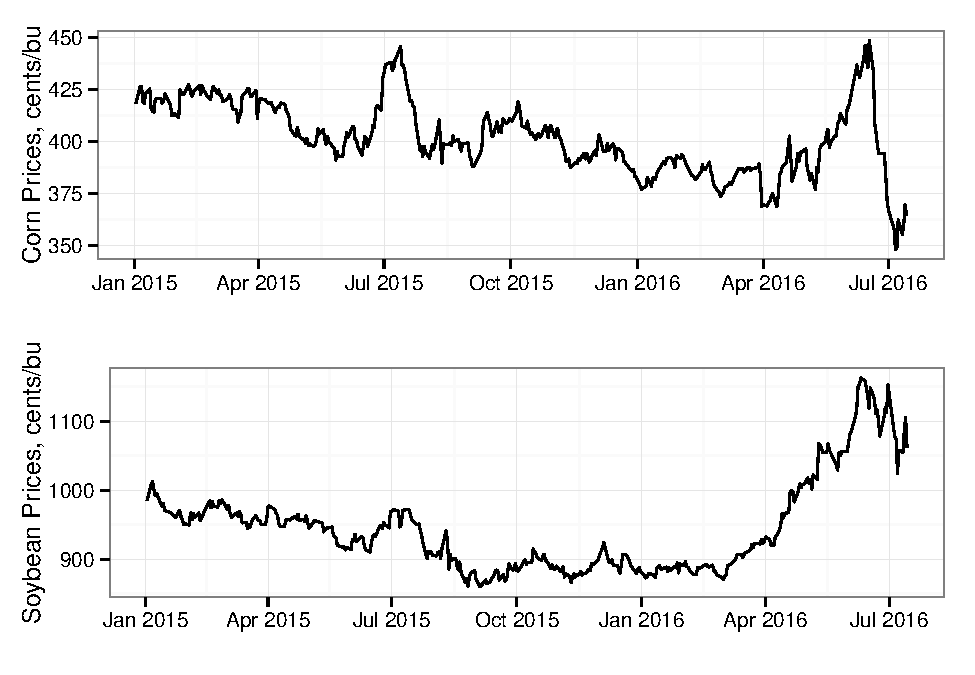
\includegraphics{manuscript-example_files/figure-latex/unnamed-chunk-4-1.pdf}

\clearpage

\section*{References}\label{references}
\addcontentsline{toc}{section}{References}

Enders, Walter. 1995. \emph{Applied Econometric Time Series}. Applied
Economic Time Series.

Said, Said E, and David A Dickey. 1984. ``Testing for Unit Roots in
Autoregressive-Moving Average Models of Unknown Order.''
\emph{Biometrika} 71 (3). Biometrika Trust: 599--607.

\end{document}


